\documentclass[conference]{IEEEtran}
\IEEEoverridecommandlockouts
\usepackage{cite}
\usepackage{amsmath,amssymb,amsfonts}
\usepackage{graphicx}
\usepackage{textcomp}
\usepackage{xcolor}
\usepackage{booktabs}
\usepackage{tikz}
\usetikzlibrary{positioning,shapes.geometric,arrows.meta,fit,calc,backgrounds}
\usepackage{pgfplots}
\pgfplotsset{compat=1.18}
\usepackage{url}

\begin{document}

\title{A Sink-Validated Python Vulnerability Detection Benchmark with Adversarial Robustness Probes}

\author{\IEEEauthorblockN{Saara Unnathi R}
\IEEEauthorblockA{\textit{Dept. of CSE} \\
\textit{RV College of Engineering}\\
Bengaluru, India \\
saaraunnathir.cs22@rvce.edu.in}
\and
\IEEEauthorblockN{Dr. Holger Schmidt}
\IEEEauthorblockA{\textit{Dept. of Computer Science} \\
\textit{Fachhochschule Dortmund}\\
Dortmund, Germany \\
holger.schmidt004@fh-dortmund.de}
\and
\IEEEauthorblockN{Dr. Klaus Kaiser}
\IEEEauthorblockA{\textit{Dept. of Computer Science} \\
\textit{Fachhochschule Dortmund}\\
Dortmund, Germany \\
klaus.kaiser@fh-dortmund.de}
}

\maketitle

\begin{abstract}
Most automated Python vulnerability detectors are evaluated on labels
inherited from CVE fix commits, where empirical audits report 25\% to 50\%
label noise from co-changed files. The CASTLE benchmark addressed this
for C/C++ with a hand-curated corpus and a static-analyzer-versus-LLM
study, but no comparable resource exists for Python. We construct a
benchmark for Python vulnerability detection covering seven sink-shaped
MITRE Top-25 CWE classes (869 samples: 440 audit-validated real-world
positives and 429 synthesized safe hard negatives). Labels are validated
by a three-layer methodology: a pre-ingest sink-presence filter, a
three-round adversarial audit by independent reviewers, and a diff-based
filter requiring the sink line itself to change between the vulnerable and
fixed versions. The combined pipeline cuts the audited false-positive rate
from 52\% to 26\%. Seven semantics-preserving mutators spanning three
families augment the benchmark and provide per-tool F1 drop as a
robustness measure. Across seven detectors in four tiers (pattern-matching
SAST, whole-project dataflow, frontier LLMs, and a fine-tuned
GraphCodeBERT), no single tool leads on every measure, and the sink-token
mutator family separates pattern-matching SAST (Bandit loses 0.187
macro-F1 under attribute-access obfuscation) from a learned detector
invariant to every mutator in the suite. All artifacts are released to
support replication.
\end{abstract}

\begin{IEEEkeywords}
vulnerability detection, benchmark, Python, label noise, adversarial
robustness, static analysis, large language models
\end{IEEEkeywords}

\section{Introduction}
Automated vulnerability detection for source code is trained and
evaluated almost entirely on C and C++. Labels come from CVE fix commits,
which typically touch several files for refactoring, tests, or cleanup
unrelated to the vulnerability. Each co-changed file silently inherits the
CVE's CWE tag, and manual audits put the resulting label noise at 25\% to
50\%~\cite{croft,cleanvul}. A benchmark built on raw CVE inheritance
therefore scores a detector's agreement with label noise as much as its
detection accuracy~\cite{primevul}.

The CASTLE benchmark~\cite{castle} addressed this for C/C++ with a
hand-curated corpus and a comparative study of static analyzers against
large language models (LLMs). No equivalent resource exists for Python,
which dominates security tooling, machine-learning pipelines, and modern
web development. A separate gap further limits existing evaluations: they
report accuracy only on unmodified code, so any published score is an
upper bound that may not survive behavior-preserving rewriting of the
input~\cite{secllmholmes}.

This paper describes a Python vulnerability-detection benchmark covering
seven sink-shaped MITRE Top-25~\cite{mitre_top25} CWE classes
(CWE-89, CWE-79, CWE-22, CWE-78, CWE-94, CWE-918, CWE-502) plus a
\emph{safe} hard-negative class. The label-noise problem is addressed with
a three-layer validation methodology that cuts the audited false-positive
rate from 52\% to 26\%, and a perpendicular robustness axis adds seven
semantics-preserving mutators, each targeting one detector shortcut.

\noindent\textbf{Contributions.}
\begin{itemize}
  \item \textbf{An audit-validated Python benchmark}: 869 samples
    (440 real-world positives plus 429 synthesized safe hard negatives)
    across seven sink-shaped CWE classes, with repo-group-stratified
    train/validation/test splits (610/127/132) and zero cross-split
    repository leakage.
  \item \textbf{A three-layer label-validation methodology}: a
    sink-presence filter, an independent adversarial audit, and a
    diff-based filter that anchors each positive on a modified sink
    line, and is to our knowledge the first sink-anchored, evidence-based
    label-validity criterion in this literature.
  \item \textbf{A robustness probe suite}: seven semantics-preserving
    mutators in three families, with a per-mutator F1-drop breakdown
    that distinguishes detectors doing real reasoning from detectors
    doing pattern matching.
  \item \textbf{A seven-detector, four-tier evaluation} showing no
    single tool dominates and that the sink-token family is the axis
    that separates pattern-matching SAST from learned detectors.
\end{itemize}

\section{Background and Related Work}

\textbf{Datasets.} Vulnerability benchmarks are dominated by C/C++:
BigVul~\cite{bigvul}, CVEfixes~\cite{cvefixes},
CrossVul~\cite{crossvul}, and DiverseVul~\cite{diversevul}
all yield few Python samples per class. Juliet~\cite{juliet} is
fully synthetic and transfers poorly to real-world code~\cite{reveal};
Devign and ReVeal~\cite{devign,reveal} are C-only. The closest
Python-specific corpus, \texttt{vudenc}~\cite{vudenc}, lacks paired fixed
versions, limiting the label validation it supports.

\textbf{Label noise.} Croft et al.~\cite{croft} audited BigVul and
reported $\approx$25\% noise; the ReVeal authors~\cite{reveal} showed
that models pick up co-changed surface cues rather than actual vulnerability
patterns. CleanVul~\cite{cleanvul} found 40\% to 75\% of labels
inaccurate across widely used datasets, and PrimeVul~\cite{primevul}
showed that a model scoring 68.3\% F1 on BigVul drops to 3.1\% on a
deduplicated, tightened-label version of the same task. D2A~\cite{d2a}
uses differential analysis for labels but operates at program rather than
sink granularity. The diff-based filter in Section~\ref{sec:dataset} is a
sink-anchored, line-level label-validity criterion.

\textbf{Detectors.} Bandit~\cite{bandit} and Semgrep~\cite{semgrep} are
single-file pattern matchers; CodeQL~\cite{codeql} performs richer
dataflow analysis but requires a compiled database with application entry
points. LLM detectors~\cite{khare_llm,steenhoek} are competitive on C/C++
but accuracy falls on real-world code. The most relevant prior work
includes CASTLE~\cite{castle} (C/C++, no robustness axis, CVE-inherited
labels), RealVuln~\cite{realvuln} (Python repositories, manual labels,
detection only), IRIS~\cite{iris} (LLM+CodeQL hybrid; its CWE-Bench-Java
targets the same sink-shaped family), and SecLLMHolmes~\cite{secllmholmes},
which demonstrated that behavior-preserving code edits reverse LLM
verdicts. Fragility of code models to such edits is well-documented
\cite{yefet,bielik,henkel}; our mutators each target one interpretable
shortcut, making per-mutator drops diagnostic rather than a single opaque
attack score.

\textbf{Positioning.} Each ingredient has precedent: large vulnerability
datasets, CVE label-noise studies, SAST-versus-LLM comparisons, and
code-model robustness work all exist in isolation. The contribution here
is their combination for Python: seven sink-shaped Top-25 CWE classes, an
automated sink-anchored label-validity criterion, and a per-mutator
robustness breakdown reported alongside detection accuracy in one
evaluation. That combination reveals which detectors reason about code
structure and which rely on surface patterns.

\section{Dataset Construction and Label Validation}
\label{sec:dataset}

The benchmark covers seven \emph{sink-shaped} CWEs, meaning classes
with a well-defined unsafe function (a ``sink'') whose misuse is the
vulnerability and whose fix modifies the sink call. Structural CWEs
(missing authorization, CSRF, etc.), which encode the \emph{absence} of
a check and require application-level context, are excluded on
methodological grounds. Positives are scraped from five advisory and
CVE-fix sources (GHSA, CVEfixes, NVD, OSV, and the \texttt{vudenc}
corpus) plus twenty hand-curated canonical exemplars.
Figure~\ref{fig:pipeline} summarizes the construction: a raw feed is
narrowed by three validation layers, with the audited false-positive
rate falling from 52\% to 26\%.

\begin{figure*}[t]
\centering
\resizebox{\textwidth}{!}{%
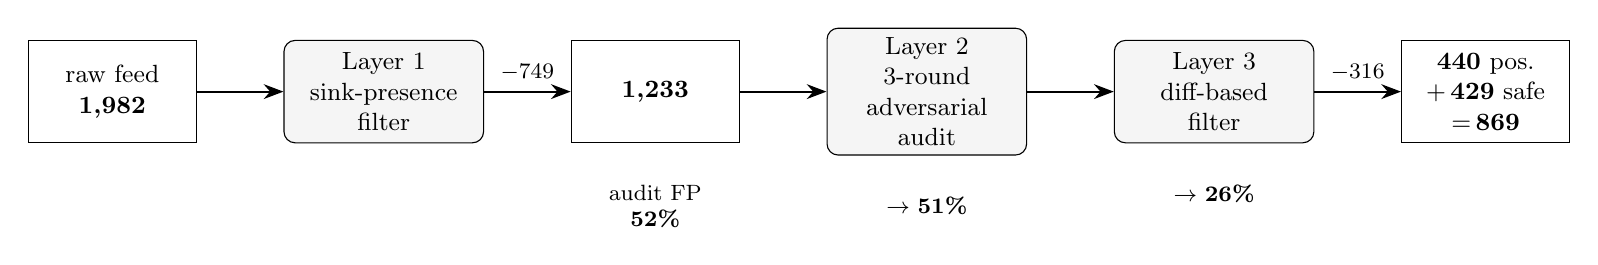
\begin{tikzpicture}[
  node distance=8mm and 11mm,
  stage/.style={draw, rounded corners, align=center, fill=gray!8,
    minimum height=13mm, text width=23mm, font=\small},
  data/.style={draw, align=center, minimum height=13mm,
    text width=19mm, font=\small},
  arr/.style={-{Stealth[length=2.5mm]}, thick},
  note/.style={font=\footnotesize, align=center}
]
\node[data] (raw) {raw feed\\\textbf{1{,}982}};
\node[stage, right=of raw] (l1) {Layer 1\\sink-presence\\filter};
\node[data, right=of l1] (d1) {\textbf{1{,}233}};
\node[stage, right=of d1] (l2) {Layer 2\\3-round\\adversarial audit};
\node[stage, right=of l2] (l3) {Layer 3\\diff-based\\filter};
\node[data, right=of l3] (final) {\textbf{440} pos.\\$+$\,\textbf{429} safe\\$=$\,\textbf{869}};
\draw[arr] (raw)--(l1);
\draw[arr] (l1)--(d1) node[midway,above,note]{$-749$};
\draw[arr] (d1)--(l2);
\draw[arr] (l2)--(l3);
\draw[arr] (l3)--(final) node[midway,above,note]{$-316$};
\node[note, below=4mm of d1] {audit FP\\\textbf{52\%}};
\node[note, below=4mm of l2] {$\rightarrow$ \textbf{51\%}};
\node[note, below=4mm of l3] {$\rightarrow$ \textbf{26\%}};
\end{tikzpicture}}
\caption{The three-layer label-validation pipeline. Layer~1 rejects
samples lacking the category-defining sink token; Layer~2's independent
audit rounds drive the pattern tightenings and the removal of two
unworkable CWE classes; Layer~3 keeps a positive only if the sink line
itself changed between the vulnerable and fixed versions. The audited
false-positive rate (measured on disjoint samples each round) falls from
52\% to 26\%.}
\label{fig:pipeline}
\end{figure*}

\subsection{Data sources}
Positives are aggregated from five primary sources with differing
retrieval methods and label quality (Table~\ref{tab:sources}). GHSA
Advisory DB dominates because it indexes per-CWE advisories with explicit
fix commits, enabling precise per-CWE scraping. The \texttt{vudenc}
corpus is human-labeled but ships no paired fixed version, so it cannot
be diff-validated and is retained as a lower-confidence tier (all
CWE-89). Twenty hand-curated canonical samples are textbook OWASP/SANS
exemplars that serve as calibration points: a detector that misses them
is broken regardless of its CVE-corpus performance.

\begin{table}[t]
\caption{Positive data sources and counts after label validation. Hard
negatives are constructed safe twins (Section~\ref{sec:dataset}).}
\label{tab:sources}
\centering
\begin{tabular}{lr l}
\toprule
\textbf{Source} & \textbf{Count} & \textbf{Retrieval} \\
\midrule
GHSA Advisory DB    & 384 & per-advisory fix commit \\
\texttt{vudenc}     & 209 & pre-labeled corpus \\
OSV / GHSA GraphQL  &  54 & commit references \\
CVEfixes            &  58 & local SQLite query \\
NVD-targeted        &  33 & NVD API + keyword filter \\
Canonical (curated) &  20 & hand-written exemplars \\
\midrule
Hard negatives      & 429 & constructed safe twins \\
\bottomrule
\end{tabular}
\end{table}

\subsection{Layer 1: sink-presence filter}
For each CWE we define a small set of regex sink patterns and admit a
sample only if at least one pattern matches its source, after stripping
comments and docstrings to suppress documentation matches. Patterns are
high-recall: they match both safe and unsafe forms of the sink, leaving
discrimination to Layer~3. Two CWEs need proximity gates (CWE-22
requires an HTTP-request reference near the sink). Applied to the 1{,}982
pre-filter samples, Layer~1 dropped 749 (38\%), with rejection rates
varying by source from 28\% (NVD) to 68\% (CVEfixes).

\subsection{Layer 2: adversarial audit}
The sink filter cannot reject a sample where the sink is present but is
not the vulnerability (co-changed-file noise). We ran three rounds of
independent audit on CWE-stratified samples. Each round samples ten
items per populous class and audits rare classes in full; for each item
the auditor receives the sample identifier, source, repository, file
path, the regex that matched, and the code excerpt around the sink, and
returns a binary correctly-labeled or mislabeled verdict with a
one-sentence justification, without seeing other auditors' verdicts.
Round~1 (77 samples)
measured a 52\% false-positive rate whose failures clustered into six
recurring patterns: sink-too-broad, co-changed-file noise,
documentation matches, pattern conflation, inverted operation, and
wrapper abstraction. Each motivated a specific pattern tightening, and
two CWEs with systematic issues (CWE-434, 100\% FP; CWE-798,
single-source bias) were dropped. Round~2 held at 51\%: pattern fixes
helped where targeted but new samples surfaced co-changed-file noise on
the untouched CWEs, motivating Layer~3.

\subsection{Layer 3: diff-based filter}
We adopt an evidence-anchored criterion: a positive is valid only if at
least one line containing a sink-pattern match differs between the
vulnerable and fixed versions (after comment stripping and whitespace
normalization). Of the 738 positives reaching Layer~3, 316 (43\%) had
unchanged sink lines and were rejected; the cut was strongly per-CWE
(CWE-79 lost 68\%, CWE-22 lost 71\%). A Round-3 audit on the
diff-filtered data measured 26\% FP, roughly halving the post-Layer-2
rate. Figure~\ref{fig:fp-progression} shows the per-CWE progression:
co-changed-file classes (CWE-502, CWE-94) collapse to 0\%, while
residual noise concentrates on CWE-89 and CWE-79, where \texttt{vudenc}
samples are retained without a paired fix to diff against.

\begin{figure}[t]
\centering
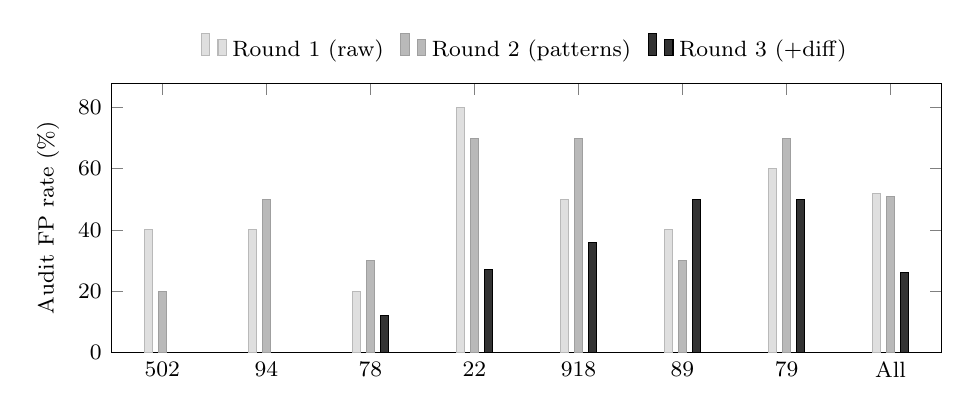
\begin{tikzpicture}
\begin{axis}[
  width=\columnwidth, height=5.0cm,
  ybar, bar width=3.0pt,
  ymin=0, ymax=88,
  ylabel={Audit FP rate (\%)},
  ylabel style={font=\footnotesize},
  symbolic x coords={502,94,78,22,918,89,79,All},
  xtick=data,
  x tick label style={font=\footnotesize},
  ytick={0,20,40,60,80},
  y tick label style={font=\footnotesize},
  legend style={at={(0.5,1.04)}, anchor=south, legend columns=3,
    font=\footnotesize, draw=none,
    /tikz/every even column/.append style={column sep=4pt}},
  enlarge x limits=0.07,
  tick align=inside,
]
\addplot+[fill=gray!25, draw=gray!55] coordinates {(502,40)(94,40)(78,20)(22,80)(918,50)(89,40)(79,60)(All,52)};
\addplot+[fill=gray!55, draw=gray!75] coordinates {(502,20)(94,50)(78,30)(22,70)(918,70)(89,30)(79,70)(All,51)};
\addplot+[fill=black!80, draw=black]   coordinates {(502,0)(94,0)(78,12)(22,27)(918,36)(89,50)(79,50)(All,26)};
\legend{Round 1 (raw), Round 2 (patterns), Round 3 ($+$diff)}
\end{axis}
\end{tikzpicture}
\caption{Per-CWE audit false-positive rate across the three validation
rounds (x-axis labels are CWE numbers; \emph{All} is the aggregate). The
diff filter collapses the co-changed-file classes to 0\% while the
residual concentrates on CWE-89 and CWE-79.}
\label{fig:fp-progression}
\end{figure}

\subsection{Hard negatives and final composition}
The 429 \texttt{safe} samples are not scraped. They are \emph{constructed
safe twins}: for each negative we take a real vulnerable function and
apply the canonical remediation for its CWE (e.g.,
\texttt{yaml.load}$\rightarrow$\texttt{yaml.safe\_load}, string-formatted
SQL$\rightarrow$parameterized query), at the AST level, preserving
surface structure and the sink \emph{name} while neutralizing only the
sink's behavior. This design gives each negative a provable safe label,
makes it a minimal-pair counterfactual that holds confounds fixed, and
targets the dominant detector failure mode directly: a tool that fires
on the mere presence of a sink token is forced into a false positive on
the twin. The final benchmark is 440 positives plus 429 safe negatives
(869 samples), split 610/127/132 with a repo-group constraint that
yields zero cross-split repository leakage (Table~\ref{tab:composition}).
Three oversized hard negatives are kept on disk but excluded from active
evaluation, leaving a 129-sample test set (67 positives, 62 negatives).

\begin{table}[t]
\caption{Final per-CWE composition.}
\label{tab:composition}
\centering
\begin{tabular}{lrrrr}
\toprule
\textbf{Label} & \textbf{Total} & \textbf{Train} & \textbf{Val} & \textbf{Test} \\
\midrule
CWE-89 (SQL Injection)             & 213 & 149 & 32 & 32 \\
CWE-502 (Insecure Deserial.)       &  75 &  52 & 11 & 12 \\
CWE-79 (XSS)                       &  54 &  40 &  7 &  7 \\
CWE-94 (Code Injection)            &  35 &  24 &  5 &  6 \\
CWE-78 (OS Command Injection)      &  26 &  18 &  4 &  4 \\
CWE-918 (SSRF)                     &  22 &  17 &  2 &  3 \\
CWE-22 (Path Traversal)            &  15 &  10 &  2 &  3 \\
\texttt{safe} (hard negatives)     & 429 & 300 & 64 & 65 \\
\midrule
\textbf{Total}                     & \textbf{869} & \textbf{610} & \textbf{127} & \textbf{132} \\
\bottomrule
\end{tabular}
\end{table}

Each sample is stored as a paired source file and a schema-versioned
metadata record carrying its CWE label, the matched sink pattern, the
provenance of the label, and CVSS severity, so that every validation
decision is reproducible from the released artifacts. Samples also carry
an implicit label-confidence tier used in stratified reporting:
\textbf{HIGH (provable)} for advisory-sourced positives whose sink line
the diff filter confirmed changed (201 of 440 positives);
\textbf{HIGH (curated)} for the 20 canonical samples, correct by
construction; and \textbf{MEDIUM (curator)} for the 209 \texttt{vudenc}
samples, which are human-labeled but lack a paired fix and so cannot be
diff-validated. The tier distinction lets a reader separate performance
on diff-anchored labels from performance on curator-labeled ones, and it
is the reason residual audit noise concentrates on CWE-89, the class the
\texttt{vudenc} tier populates.

\section{Adversarial Robustness Methodology}
\label{sec:method}

Beyond binary detection accuracy, we generate seven semantics-preserving
variants of every test sample to probe robustness. Each variant rewrites
the code so that runtime behavior is unchanged but a specific detector
shortcut is disabled; a sharp F1 drop on a given mutator identifies the
shortcut that tool relied on. The mutators operate on the Python AST and
are deterministic given a sample identifier and seed, making the
evaluation reproducible. Each mutator satisfies three properties:
\emph{semantics-preserving} (when a transformation cannot be proven safe,
such as a rename that might collide with an imported name, the mutator
skips that node); \emph{targeted} at one specific shortcut rather than
generic obfuscation, so per-mutator F1 drops are diagnostic; and
\emph{realistic}, meaning identifiers become synonyms and dead code reads
like ordinary scaffolding rather than adversarial gibberish. The mutators
fall into three families (Figure~\ref{fig:mutator-tax}).

\begin{figure}[t]
\centering
\resizebox{\columnwidth}{!}{%
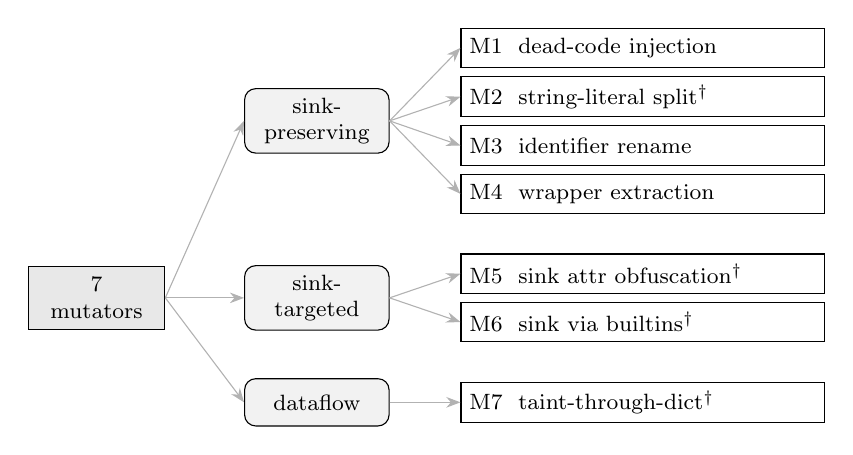
\begin{tikzpicture}[
  font=\footnotesize,
  root/.style={draw, fill=gray!18, align=center, text width=15mm, minimum height=8mm},
  fam/.style={draw, rounded corners, fill=gray!10, align=center, text width=16mm, minimum height=6mm},
  leaf/.style={draw, align=left, text width=44mm, minimum height=5mm, inner sep=3pt},
  arr/.style={-{Stealth[length=1.8mm]}, gray!60},
]
\node[leaf] (m1) {M1\ \ dead-code injection};
\node[leaf, below=1mm of m1] (m2) {M2\ \ string-literal split$^{\dagger}$};
\node[leaf, below=1mm of m2] (m3) {M3\ \ identifier rename};
\node[leaf, below=1mm of m3] (m4) {M4\ \ wrapper extraction};
\node[leaf, below=5mm of m4] (m5) {M5\ \ sink attr obfuscation$^{\dagger}$};
\node[leaf, below=1mm of m5] (m6) {M6\ \ sink via builtins$^{\dagger}$};
\node[leaf, below=5mm of m6] (m7) {M7\ \ taint-through-dict$^{\dagger}$};
\node[fam, anchor=east] (f1) at ($(m1.west)!0.5!(m4.west) + (-9mm,0)$) {sink-\\preserving};
\node[fam, anchor=east] (f2) at ($(m5.west)!0.5!(m6.west) + (-9mm,0)$) {sink-\\targeted};
\node[fam, anchor=east] (f3) at ($(m7.west) + (-9mm,0)$) {dataflow};
\node[root, anchor=east] (r) at ($(f2.west) + (-10mm,0)$) {7\\mutators};
\draw[arr] (r.east) -- (f1.west);
\draw[arr] (r.east) -- (f2.west);
\draw[arr] (r.east) -- (f3.west);
\foreach \l in {m1,m2,m3,m4} \draw[arr] (f1.east) -- (\l.west);
\foreach \l in {m5,m6} \draw[arr] (f2.east) -- (\l.west);
\draw[arr] (f3.east) -- (m7.west);
\end{tikzpicture}}
\caption{The seven mutators grouped by the detector shortcut each family
probes. Mutators marked $\dagger$ are held out of training-time
augmentation and used only as test-time robustness probes.}
\label{fig:mutator-tax}
\end{figure}

The \emph{sink-preserving} family (M1--M4: dead-code injection, string
splitting, identifier rename, wrapper extraction) alters code around the
sink but leaves the sink identifier and the arguments reaching it
intact, probing positional, substring, identifier-memorization, and
single-function shortcuts. The \emph{sink-targeted} family rewrites the
sink call itself: M5 turns \texttt{os.system(x)} into
\texttt{getattr(os,"system")(x)} (CWE-78/89/918/502) and M6 turns
\texttt{eval(x)} into \texttt{\_\_import\_\_("builtins").\_\_dict\_\_["eval"](x)}
(CWE-94), so the sink token survives only inside a string literal. The
\emph{dataflow} family (M7) leaves both intact and routes the sink's
first argument through a one-entry dict (\texttt{f(\{"a":x\}["a"])}),
breaking the static lineage from parameter to sink argument. At
evaluation time we apply two to three mutators per sample and also report
each mutator in isolation. Every mutated sample must re-parse, and the
per-node transformations are individually semantics-preserving under the
Python evaluation rules.

\section{Evaluation}
\label{sec:eval}

The evaluation answers three questions. \textbf{RQ1:} how accurately do
the detectors classify the seven sink-shaped CWE classes on clean code?
\textbf{RQ2:} how does each detector's accuracy change under a
semantics-preserving mutator, and which mutator exposes the most
brittleness? \textbf{RQ3:} does the diff-based label filter change the
picture a detector evaluation paints? We do not rank detectors; the
purpose is to demonstrate what the benchmark measures.

\subsection{Setup}
The held-out test set is 129 samples (67 positives across the seven
classes, 62 \texttt{safe} negatives). We score every detector one-vs-rest
per CWE and report five bounded measures: macro-F1 across the seven
classes; detection MCC~\cite{chicco2020mcc} on the binary
vulnerable-versus-safe collapse; Severity-Weighted Recall (SWR), the
CVSS-weighted recall on the 27 CVSS-scored positives; Hierarchical CWE
Macro-Accuracy (HCMA), which gives Wu--Palmer~\cite{wupalmer1994} partial
credit for close-sibling confusions on a hand-coded CWE subtree; and
weighted Cohen's $\kappa$~\cite{cohen1968kappa}. The five answer separate
questions (CWE identification, binary detection, severity-weighted
recall, hierarchical near-miss credit, and chance-corrected agreement)
and are reported jointly rather than collapsed into a single composite
score, so a reader can see exactly where a detector is strong: macro-F1
matters because class sizes range from 3 to 32, MCC because the clean set
is roughly balanced, and SWR because not all positives carry equal
severity. The robustness drop is clean macro-F1 minus mutated macro-F1,
computed over the 67 positives so the subtraction is like-for-like. We evaluate seven detectors across four
tiers (Figure~\ref{fig:harness}): pattern-matching SAST (Bandit~1.9.4,
Semgrep~1.163.0), whole-project dataflow (Snyk Code~1.1305.0; CodeQL was
attempted), frontier LLMs (Claude Sonnet~4.6, GPT-4o, DeepSeek~R1), and a
fine-tuned GraphCodeBERT~\cite{graphcodebert} classifier trained on the
benchmark split.

\begin{figure}[t]
\centering
\resizebox{\columnwidth}{!}{%
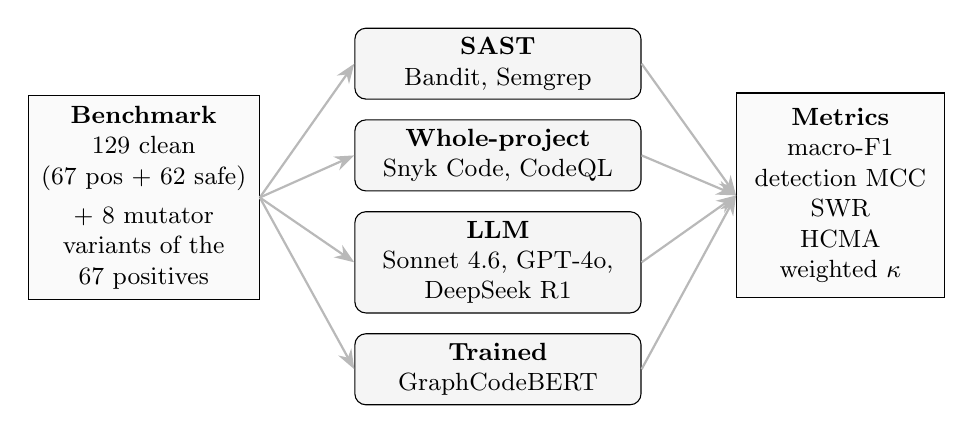
\begin{tikzpicture}[
  font=\small,
  box/.style={draw, rounded corners, align=center, fill=gray!8,
    minimum height=9mm, text width=34mm},
  src/.style={draw, align=center, fill=gray!4, minimum height=26mm,
    text width=27mm},
  met/.style={draw, align=center, fill=gray!4, minimum height=26mm,
    text width=24mm},
  arr/.style={-{Stealth[length=2.5mm]}, thick, gray!55},
]
\node[src] (bench) {\textbf{Benchmark}\\129 clean\\(67 pos $+$ 62 safe)\\[3pt]$+$ 8 mutator\\variants of the\\67 positives};
\node[box, right=12mm of bench, yshift=17mm] (sast) {\textbf{SAST}\\Bandit, Semgrep};
\node[box, below=2.5mm of sast] (wp) {\textbf{Whole-project}\\Snyk Code, CodeQL};
\node[box, below=2.5mm of wp] (llm) {\textbf{LLM}\\Sonnet 4.6, GPT-4o,\\DeepSeek R1};
\node[box, below=2.5mm of llm] (trained) {\textbf{Trained}\\GraphCodeBERT};
\node[met, right=12mm of llm, yshift=8.5mm] (metrics) {\textbf{Metrics}\\macro-F1\\detection MCC\\SWR\\HCMA\\weighted $\kappa$};
\draw[arr] (bench.east) -- (sast.west);
\draw[arr] (bench.east) -- (wp.west);
\draw[arr] (bench.east) -- (llm.west);
\draw[arr] (bench.east) -- (trained.west);
\draw[arr] (sast.east) -- (metrics.west);
\draw[arr] (wp.east) -- (metrics.west);
\draw[arr] (llm.east) -- (metrics.west);
\draw[arr] (trained.east) -- (metrics.west);
\end{tikzpicture}}
\caption{The evaluation harness: the same 129-sample clean set and eight
mutator variants of the 67 positives are scored against seven detectors
in four tiers under five bounded metrics.}
\label{fig:harness}
\end{figure}

\subsection{Headline results}
Table~\ref{tab:headline} reports the seven detectors. \emph{No single
tool leads on every measure.} DeepSeek~R1 narrowly leads macro-F1
(0.596); Sonnet~4.6 leads SWR (0.903) and HCMA (0.805); the trained
GraphCodeBERT leads detection MCC ($+0.556$); and Bandit edges weighted
$\kappa$ ($+0.567$). The two LLMs Sonnet and GPT-4o sit far below the
SAST and learned tiers on MCC because they over-flag hard negatives as
CWE-22 and CWE-918. Snyk Code is an outlier on every detection metric
(macro-F1 0.063); we treat its row as a methodological signal rather than
a ranking, discussed in Section~\ref{sec:eval:shape}.

The hierarchical and agreement columns sharpen the comparison between
Bandit and the trained detector. On macro-F1 Bandit (0.510) trails
GraphCodeBERT (0.524) by 0.014, but on HCMA the gap inverts and Bandit
(0.564) edges ahead (0.547). The mechanism is visible in the confusions:
Bandit's errors are dominated by close-sibling mistakes inside the
injection subtree (CWE-94 flagged as CWE-78, and the reverse), which
Wu--Palmer credits as partial matches but macro-F1 scores as flat misses,
whereas GraphCodeBERT's confusions are more diffuse and benefit less from
partial credit. Weighted $\kappa$ converges on the same conclusion:
Bandit ($+0.567$) and GraphCodeBERT ($+0.548$) are within 0.019 of each
other and both lead Semgrep by more than 0.30. The single-number reading
is that Bandit and the trained detector are comparable on clean code
under any partial-credit metric; the trained detector's headline win is
most visible on SWR and disappears on chance-corrected agreement.

\begin{table*}[t]
\caption{Detector results on the 129-sample clean test set. Macro-F1 is
one-vs-rest across seven CWEs; MCC is on the binary vulnerable/safe
collapse; SWR is severity-weighted recall on the 27 CVSS-scored
positives; HCMA is hierarchical accuracy; $\kappa_w$ is weighted Cohen's
$\kappa$; Comp.\ is macro-F1 on the composed mutator; $\Delta$F1$^\star$
is the worst-case single-mutator drop (positives only).}
\label{tab:headline}
\centering
\begin{tabular}{lrrrrrrr}
\toprule
\textbf{Detector} & \textbf{macro-F1} & \textbf{MCC} & \textbf{SWR} & \textbf{HCMA} & $\boldsymbol{\kappa_w}$ & \textbf{Comp.} & $\boldsymbol{\Delta}$\textbf{F1}$^{\star}$ \\
\midrule
Bandit               & 0.510 & $+0.478$ & 0.745 & 0.564 & $\mathbf{+0.567}$ & 0.589 & $+0.187$ \\
Semgrep              & 0.315 & $+0.157$ & 0.634 & 0.353 & $+0.227$ & 0.375 & $+0.132$ \\
Snyk Code            & 0.063 & $-0.235$ & 0.143 & 0.069 & $-0.097$ & 0.088 & $+0.036$ \\
Claude Sonnet 4.6    & 0.585 & $+0.117$ & $\mathbf{0.903}$ & $\mathbf{0.805}$ & $+0.396$ & 0.867 & $0.000$ \\
GPT-4o               & 0.356 & $+0.047$ & 0.420 & 0.419 & $+0.295$ & 0.565 & $+0.026$ \\
DeepSeek R1          & $\mathbf{0.596}$ & $+0.410$ & 0.691 & 0.646 & $+0.539$ & 0.567 & $+0.068$ \\
GraphCodeBERT (ours) & 0.524 & $\mathbf{+0.556}$ & 0.870 & 0.547 & $+0.548$ & 0.603 & $0.000$ \\
\bottomrule
\end{tabular}
\end{table*}

\subsection{Detection on clean code (RQ1)}
Among the SAST and learned tiers, detectors diverge most on SQL
injection: Bandit reaches F1 0.80 on CWE-89 by lexically matching inline
SQL, GraphCodeBERT 0.63, and Semgrep only 0.06 because its taint-shape
rules require a framework-recognizable source-to-sink shape absent from
the fragmentary \texttt{vudenc} samples. CWE-22 scores zero for all three
(no usable rule; too few training samples), and CWE-918 separates the
tiers: both SAST tools score zero while GraphCodeBERT recovers F1 0.57.
The macro-average deliberately reports the CWE-22 gap rather than
averaging it away. Table~\ref{tab:clean-percwe} gives the per-class
breakdown; restricted to the 67 positives the same detectors score
0.59, 0.38, and 0.57, and the gap to the all-129 macro-F1 is the F1 cost
of false positives on the safe class, which is smallest for the trained
detector (0.05) and largest for Bandit (0.08).

\begin{table}[t]
\caption{Per-CWE F1 on the clean test set ($n$ = positive test samples).
GCB is the trained GraphCodeBERT detector.}
\label{tab:clean-percwe}
\centering
\begin{tabular}{lrrrr}
\toprule
\textbf{CWE} & $n$ & \textbf{Bandit} & \textbf{Semgrep} & \textbf{GCB} \\
\midrule
CWE-22  Path Traversal       &  3 & 0.00 & 0.00 & 0.00 \\
CWE-78  OS Command Injection &  4 & 0.38 & 0.29 & 0.40 \\
CWE-79  Cross-site Scripting &  7 & 0.60 & 0.33 & 0.67 \\
CWE-89  SQL Injection        & 32 & 0.80 & 0.06 & 0.63 \\
CWE-94  Code Injection       &  6 & 0.92 & 0.80 & 0.57 \\
CWE-502 Insecure Deserial.   & 12 & 0.83 & 0.73 & 0.83 \\
CWE-918 SSRF                 &  3 & 0.00 & 0.00 & 0.57 \\
\midrule
Macro-F1 (positives $+$ safe) &   & 0.51 & 0.32 & 0.52 \\
\bottomrule
\end{tabular}
\end{table}

\subsection{Adversarial robustness (RQ2)}
The families separate the tiers sharply (Table~\ref{tab:robustness}). The
two pattern-matching SAST tools show a robustness \emph{cliff} on the
sink-targeted family: Bandit drops 0.187 macro-F1 under attribute
obfuscation (a 47\% relative loss in severity-weighted recall) and 0.143
under builtins indirection; Semgrep drops 0.109 and 0.132. The cliff
replicates across two mutators attacking disjoint sink classes, so it is
a property of lexical sink-matching rather than a single trick. The
trained GraphCodeBERT detector is invariant to every mutator
($|\Delta\textrm{F1}|\le0.036$), as are all three LLMs (worst-case drops
$0.000$, $+0.026$, $+0.068$). All detectors are invariant to the four
sink-preserving mutators and to the dataflow mutator. The dataflow
result holds because none of the current detectors performs dataflow
analysis, so M7 remains a coverage slot for future dataflow-aware tools.

\begin{table}[t]
\caption{Macro-F1 by variant over the 67 positives. DC/SS/VR/WE:
sink-preserving; SAO/SVG: sink-targeted; TTD: dataflow; Comp: composed.}
\label{tab:robustness}
\centering
\setlength{\tabcolsep}{3.0pt}
\resizebox{\columnwidth}{!}{%
\begin{tabular}{lrrrrrrrrr}
\toprule
\textbf{Tool} & \textbf{Clean} & DC & SS & VR & WE & SAO & SVG & TTD & Comp \\
\midrule
Bandit        & 0.59 & 0.59 & 0.59 & 0.59 & 0.59 & 0.40 & 0.45 & 0.59 & 0.58 \\
Semgrep       & 0.38 & 0.38 & 0.38 & 0.38 & 0.38 & 0.28 & 0.25 & 0.37 & 0.38 \\
GraphCodeBERT & 0.57 & 0.59 & 0.60 & 0.60 & 0.61 & 0.60 & 0.57 & 0.60 & 0.60 \\
\bottomrule
\end{tabular}}
\end{table}

The central robustness finding is the contrast between the three
families: a mutator must target sink \emph{syntax} to expose brittleness
in pattern-matching SAST; semantic features beyond the sink identifier
carry the learned detector through that axis; and the dataflow axis marks
where a robustness cliff would appear for a future generation of
dataflow-aware detectors, which the current work does not evaluate. Table~\ref{tab:drop} reports the drops grouped by family in
both macro-F1 and severity-weighted recall; the SAST cliff is visible on
the sink-targeted columns (Bandit loses up to 0.347 SWR) and absent
everywhere on the learned detector.

\begin{table}[t]
\caption{Robustness drop (clean $-$ mutator) by family. Sink-preserve is
the mean of the four sink-preserving mutators; SAO, SVG, and TTD are
individual. $\Delta$SWR is the drop in severity-weighted recall.}
\label{tab:drop}
\centering
\setlength{\tabcolsep}{3.0pt}
\resizebox{\columnwidth}{!}{%
\begin{tabular}{lrrrrrrrr}
\toprule
& \multicolumn{2}{c}{Sink-preserve} & \multicolumn{2}{c}{SAO} & \multicolumn{2}{c}{SVG} & \multicolumn{2}{c}{TTD} \\
\cmidrule(lr){2-3}\cmidrule(lr){4-5}\cmidrule(lr){6-7}\cmidrule(lr){8-9}
\textbf{Tool} & $\Delta$F1 & $\Delta$SWR & $\Delta$F1 & $\Delta$SWR & $\Delta$F1 & $\Delta$SWR & $\Delta$F1 & $\Delta$SWR \\
\midrule
Bandit        & $+$.001 & .000  & $+$.187 & $+$.347 & $+$.143 & $+$.246 & .000  & .000 \\
Semgrep       & $+$.005 & .000  & $+$.109 & $+$.196 & $+$.132 & $+$.246 & $+$.018 & $-$.029 \\
GraphCodeBERT & $-$.036 & $+$.009 & $-$.035 & $+$.034 & .000  & .000  & $-$.030 & .000 \\
\bottomrule
\end{tabular}}
\end{table}

\subsection{LLM detectors}
The three LLMs separate sharply. \textbf{DeepSeek~R1} posts the highest
macro-F1 in the table (0.596) and the highest CWE-89 F1 of any detector
(0.935); its MCC ($+0.410$) is by far the best of the three LLMs,
indicating its CWE assignments and binary verdict agree more often than
the others'. \textbf{Sonnet~4.6} ranks just below on macro-F1 (0.585)
and takes the SWR (0.903) and HCMA (0.805) leads of the entire table,
but its MCC ($+0.117$) is low because it over-flags hard negatives as
CWE-22 (15 false positives) and CWE-918 (17). \textbf{GPT-4o} is the
weakest LLM (macro-F1 0.356, MCC $+0.047$ near chance): it reaches F1
0.915 on CWE-89 but scores zero on CWE-94 and over-applies CWE-22 and
CWE-918 to safe code, a miscalibration rather than a uniform weakness.
All three are essentially invariant to the mutators, confirming that the
sink-token cliff is a property of lexical SAST, not of the mutator suite.

\subsection{Trained-model detector}
The 610-sample training split fine-tunes a dual-task
GraphCodeBERT~\cite{graphcodebert} that predicts the CWE class and CVSS
base score, using a three-phase schedule (supervised-contrastive warmup,
LDAM~\cite{cao2019ldam} margin loss on a class-balanced sampler, then
deferred re-weighting with Effective-Number~\cite{cui2019cb} weights).
Three of the seven mutators are applied as online augmentation; the other
four are held out as test-time probes. The detector reaches macro-F1
0.524 and the table-leading detection MCC ($+0.556$), reflecting a lower
false-positive rate on hard negatives than either SAST tool or any LLM.
We treat this as a defensible small-data existence proof (610 samples is
small for a 126.6M-parameter model) that a benchmark-tuned learned
detector can compete with mature SAST baselines and frontier LLMs on
Python sink-shaped CWEs, not as a state-of-the-art or
generalization claim.

\subsection{Whole-project dataflow detectors}
\label{sec:eval:shape}
Snyk Code is built for whole-application analysis but is scored here on
single-function extracts; it flags 1 of 32 CWE-89 positives and produces
many false positives on the safe class, because the framework
source-to-sink lineage it tracks is absent from the extracts. CodeQL
returned \emph{zero} findings for the same reason: its source model
requires application entry points (Flask routes, Django views) the
extracts do not contain. We read this as a property of the benchmark
\emph{format}, not the tools, and keep both detector implementations in
the released harness for future application-level benchmarks. The Snyk
Code row appears in Table~\ref{tab:headline} to make the bound
empirically visible.

\subsection{Effect of the label filter (RQ3)}
The numbers above use the diff-filtered labels (26\% audited FP). Run
against unfiltered labels, every tool's apparent precision falls by
construction, because a tool that correctly declines a mislabeled sample
is charged a false negative. The filter therefore does not flatter the
tools; it removes samples on which a correct detector and a wrong label
disagree.

\section{Threats to Validity and Limitations}
The limitations below follow the standard construct, internal, external,
and conclusion validity categories. Each represents residual exposure that
a downstream user of the benchmark should weigh against the headline
results.

\subsection{Construct validity}
We do not claim a noise-free label set. An absolute score reported on
this benchmark inherits the 26\% audited residual and should not be read
as a tool's true accuracy on a hypothetical clean corpus; the
\emph{between}-tool comparison on the same labels is the robust reading,
since both tools score against the same residual. A second concern is
that the sink-presence filter is itself a definition of what counts as a
correct label, so a detector that uses the same sink regexes inherits a
measurement advantage. We release the full pattern set, the audit
reports for all three rounds, and a per-sample rejection manifest with
reason codes so this dependence is auditable rather than hidden. A third
concern is the strength of the mutator suite: all seven mutators are
semantics-preserving by AST-level construction, but one sink-targeted
axis (dynamic dispatch through a runtime-variable attribute name) is not
yet exercised and could reveal an axis on which the learned detector is
not invariant.

\subsection{Internal validity}
Single-CVE clustering, in which one high-impact CVE generates several
near-identical files, is mitigated by a per-CVE sample cap of three and
by the repo-group split constraint, which forces samples sharing a
repository into the same split; we verify zero cross-split repository
leakage. The evaluation uses one splitter seed and one run per detector.
This is sound for the deterministic SAST tools and the fixed-checkpoint
GraphCodeBERT, and the LLMs run at temperature~0 or with the temperature
removed, so per-call drift is small but not bit-for-bit zero.

\subsection{External validity}
The benchmark is Python-specific; the validation methodology is
language-agnostic in design but the sink pattern set would need
re-deriving for another language. It is also limited to sink-shaped
CWEs, so a detector that handles structural CWEs well is not measurable
here, and the scores are not a comprehensive Python ranking. The scraped
corpus over-represents popular projects (Django, Flask, FastAPI) and
under-represents small or unmaintained ones; the 20 canonical samples
only partly offset this. Finally, the single-file extract format is
unfavorable to whole-project dataflow detectors (Section~\ref{sec:eval:shape}).

\subsection{Conclusion validity}
The 129-sample test set is small by post-PrimeVul standards. Per-class
F1 intervals are wide for CWE-22, CWE-78, and CWE-918, where the
positive count is below seven and a single prediction flip moves F1 by
14 to 33 points, and the 67-positive mutator subset gives a per-sample
F1 swing of about 1.5\%, so an absolute macro-F1 change below 0.04 lies
near the noise floor and should not be read as a signed result. The SVG
mutator applies to only 6 positives (all CWE-94 \texttt{eval} sinks), so
its drop confirms the direction of the SAO cliff rather than standing
alone. The learned-detector invariance is a property of one
GraphCodeBERT checkpoint, not of learned detectors in general. A
multi-seed, multi-model protocol with paired bootstrap intervals is the
planned follow-up; until it is run, the robustness conclusions are
scoped to the detectors evaluated here.

\section{Conclusion}
This paper presented an audit-validated Python vulnerability-detection
benchmark of 869 samples across seven sink-shaped CWE classes. A
three-layer label-validation methodology cuts the audited false-positive
rate from 52\% to 26\%, and a diff-based filter anchors each positive on
a modified sink line. Seven semantics-preserving mutators extend the
benchmark to a joint detection-and-robustness evaluation. Across seven
detectors in four tiers, no single tool leads on every measure; the
sink-token mutator family separates pattern-matching SAST (up to 0.187
macro-F1 drop) from a learned detector invariant to every mutator. All
artifacts, audit reports, rejection manifests, and tool runners are
released to support replication and extension to additional languages,
CWE classes, and dataflow-aware detectors at the application level.

\bibliographystyle{IEEEtran}
\bibliography{bib/references}

\end{document}
